%
% abbildungen.tex -- Lineare Abbildungen
%
% (c) 2018 Prof Dr Andreas Müller, Hochschule Rapperswil
%
\section{Lineare Abbildungen%
\label{skript:section:lineare abbildungen}}
Wie im vorangegangenen Abschnitt verwenden wir im folgenden eine Basis
$\mathcal{B}=\{\vec{b}_1,\dots,\vec{b}_n\}$, die Vektoren $\vec{v}_i$
sind linear unabhängig, und jeder Vektor lässt sich als Linearkombination
dieser Basisvektoren schreiben.

%
% Affine Abbildungen
%
\subsection{Affine und lineare Abbildungen}
Wenn man von einem Problem einen Plan machen, dann darf die Perspektive
keine Rolle spielen.
Der Plan darf keine für das Problem wesentlichen Eigenschaften stören.
Auf ein mathematisches Problem übertragen müssen wir in der Lage sein,
Abbildungen auf das Problem anzuwenden, welche helfen können, das
Problem zu lösen.
Diese Abbildungen dürfen die wesentlichen Eigenschaften der untersuchten
Objekte nicht verändern.

Die dem Abschnitt~\ref{skript:koordinaten} vorangestellten Axiome
sprechen von Geraden, Ebenen und Parallelen als den primären geometrischen
Objekten.
Zulässige Abbildungen dürfen also Ebenen und Geraden nicht zerstören.
Wenn aber Geraden auf Geraden abgebildet werden, dann werden Geraden,
die sich nicht schneiden, auf Geraden abgebildet, die sich nicht schneiden,
Parallelität ist also automatisch erhalten.

\begin{definition}
Eine Abbildung, die Ebene, Geraden und Parallelität erhält,
heisst {\em affine Abbildung}
\end{definition}
\index{affine Abbildung}

Aus den Axiomen haben wir die algebraischen Eigenschaften von Ortsvektoren
konstruiert.
Affine Abbildungen müssen also verträglich sein mit den algebraischen
Operationen.
Um die Geometrie mit Vektoren auszudrücken, mussten wir ausserdem
einen ausgezeichneten Punkt $O$ haben.
Dieser muss natürlich unter Abbildungen, die uns interessieren
ebenfalls erhalten bleiben.
Eine affine Abbildung $\varphi$ muss also folgende Regeln erfüllen:
\begin{align*}
\varphi(O)&=O
\\
\varphi(\lambda\vec{p})&=\lambda\varphi(\vec{p})
\\
\varphi(\vec{u}+\vec{v})&=\varphi(\vec{u}) + \varphi(\vec{v})
\end{align*}

\begin{definition}
Eine Abbildung $\varphi\colon \mathbb R^n \to \mathbb R^m$ mit den
Eigenschaften
\begin{align*}
\varphi(\lambda\vec{p})&=\lambda\varphi(\vec{p})
&&\text{und}&
\varphi(\vec{u}+\vec{v})&=\varphi(\vec{u}) + \varphi(\vec{v})
\end{align*}
heisst {\em linear}.
\end{definition}

%
% Beschreibung linearer Abbildungen mit Matrizen
%
\subsection{Beschreibung linearer Abbildungen mit Matrizen}
Wir wollen jetzt lineare Abbildungen der Ebene und des dreidimensionalen
Raumes mit Hilfe einer Basis genauer beschreiben.
Sei also eine Basis $\mathcal{B}=\{\vec{b}_1,\dots,\vec{b}_n\}$ 
gegeben und eine lineare Abbildung $\varphi$.

\subsubsection{Matrix einer linearen Abbildung}
Jeder beliebige Vektor $\vec{x}$ kann als Linearkombination
\[
\vec{x}
=
x_1\vec{b}_1
+\dots+
x_n\vec{b}_n
\]
der Vektoren $\vec{b}_i$ geschrieben werden.
Der Bildvektor $\varphi(\vec{x})$ kann mit den Linearitätseigenschaften
vereinfacht werden:
\[
\varphi(\vec{x})
=
\varphi(
x_1\vec{b}_1
+\dots+
x_n\vec{b}_n
)
=
x_1\varphi(\vec{b}_1)
+\dots+
x_n\varphi(\vec{b}_n).
\]
Die lineare Abbildung ist also vollständig durch die Bilder der Basisvektoren
$\varphi(\vec{b}_i)$ festgelegt.

In der Basis werden die Vektoren $\vec{b}_i$ durch die Standardbasisvektoren
\[
\vec{e}_1 = \begin{pmatrix}1\\0\\\vdots\\0\end{pmatrix},\quad
\vec{e}_2 = \begin{pmatrix}0\\1\\\vdots\\0\end{pmatrix},
\quad\dots,\quad
\vec{e}_n = \begin{pmatrix}0\\0\\\vdots\\1\end{pmatrix}
\]
dargestellt.
Auch die Bildvektoren können in der Basis $\mathcal{B}$ ausgedrückt werden,
wir schreiben die Bilder als Spaltenvektoren
\[
\vec{a}_i
=
\varphi(\vec{b}_i)
=
\begin{pmatrix}
a_{1i}\\a_{2i}\\\vdots\\a_{ni}
\end{pmatrix}.
\]
Der Bildvektor $\varphi(\vec{x})$ ist daher die Linearkombination
\[
\varphi(\vec{x})
=
x_1
\begin{pmatrix}
a_{11}\\a_{21}\\\vdots\\a_{n1}
\end{pmatrix}
+
x_2
\begin{pmatrix}
a_{12}\\a_{22}\\\vdots\\a_{n2}
\end{pmatrix}
+
\dots
+
x_n
\begin{pmatrix}
a_{1n}\\a_{2n}\\\vdots\\a_{nn}
\end{pmatrix}
=
\begin{pmatrix}
a_{11}&a_{12}&\dots &a_{1n}\\
a_{21}&a_{22}&\dots &a_{2n}\\
\vdots&\vdots&\ddots&\vdots\\
a_{21}&a_{22}&\dots &a_{2n}
\end{pmatrix}
\begin{pmatrix}
x_1\\x_2\\\vdots\\x_n
\end{pmatrix}
\]
Die Spalten der Matrix $A$ sind die Koordinatenvektoren der Bilder
$\varphi(\vec{b}_i)$.
Wir fassen diese Resultate wie folgt zusammen.

\begin{satz}
\label{satz:affin:bilderderstandardbasisvektoren}
Eine lineare Abbildung wird durch die Matrix $A$ vollständig beschrieben,
die Spalten enthalten die Bilder der Standardbasisvektoren.
\end{satz}

\subsubsection{Beispiel: Matrix einer Spiegelung}
\begin{figure}
\centering
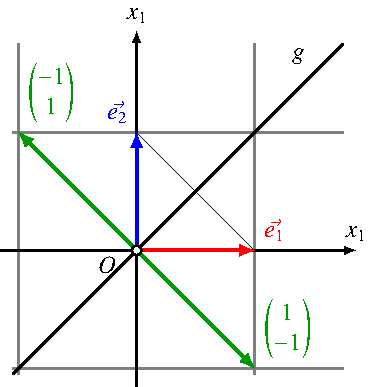
\includegraphics{3/images/spiegelung.pdf}
\caption{Die Spiegelung an der Geraden $g$ bildet den Vektor
$\vec{e}_1$ auf $\vec{e}_2$ ab und umgekehrt.
\label{skript:affin:spiegelung}}
\end{figure}
Wir suchen die Matrix einer Spiegelung der Ebene an der Geraden durch
die Punkte $O$ und $(2,2)$.
Nach Satz~\label{satz:affin:bilderderstandardbasisvektoren} müssen wir 
die Bilder der Standardbasisvektoren bestimmen.
Aus Abbildung~\ref{skript:affin:spiegelung} kann man ablesen, dass die
Spiegelung den Vektor $\vec{e}_1$ auf $\vec{e}_2$ abbildet und umgekehrt.
Daraus kann man jetzt die Matrix $S$ der Spiegelung zusammensetzen,
sie enthält die Bilder der Standardbasisvektoren:
\[
\vec{e}_1\leftrightarrow\vec{e}_2
\qquad\Leftrightarrow\qquad
\begin{pmatrix}1\\0\end{pmatrix}
\leftrightarrow
\begin{pmatrix}0\\1\end{pmatrix}
\qquad\Leftrightarrow\qquad
S
=
\begin{pmatrix}0&1\\1&0\end{pmatrix}.
\]
Wir kontrollieren dieses Resultate, indem wir berechnen wie ein Vektor
auf der Geraden und senkrecht dazu abgebildet wird:
\begin{align*}
S
\begin{pmatrix}1\\1\end{pmatrix}
&=
\begin{pmatrix}0&1\\1&0\end{pmatrix}
\begin{pmatrix}1\\1\end{pmatrix}
=
\begin{pmatrix}1\\1\end{pmatrix}
\\
S
\begin{pmatrix}1\\-1\end{pmatrix}
&=
\begin{pmatrix}0&1\\1&0\end{pmatrix}
\begin{pmatrix}1\\-1\end{pmatrix}
=
\begin{pmatrix}-1\\1\end{pmatrix}
=
-
\begin{pmatrix}1\\-1\end{pmatrix}.
\end{align*}
Der Vektor in der zweiten Zeile steht senkrecht auf der Geraden $g$ 
und wird durch die Spiegelung mit $-1$ multipliziert.

\subsubsection{Beispiel: Matrix einer Drehung}
\begin{figure}
\centering
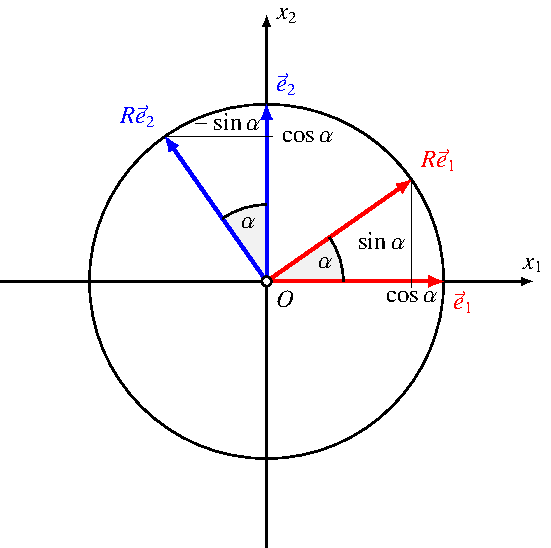
\includegraphics{3/images/drehung.pdf}
\caption{Drehung der Ebene um den Winkel $\alpha$.
Die Drehmatrix $R$ besteht aus den Bildern der Standardbasisvektoren.
\label{skript:affin:drehung}}
\end{figure}
Gesucht ist die Matrix $R$ einer Drehung um den Winkel $\alpha$.
Aus Abbildung~\ref{skript:affin:drehung} liest man die Bilder der
Standardbasisvektoren ab:
\[
R\colon \vec{e}_1 \mapsto \begin{pmatrix}\cos\alpha\\\sin\alpha\end{pmatrix},
\qquad
R\colon \vec{e}_2 \mapsto \begin{pmatrix}-\sin\alpha\\\cos\alpha\end{pmatrix}.
\]
Daraus kann man die Drehmatrix
\[
R=\begin{pmatrix}\cos\alpha&-\sin\alpha\\\sin\alpha&\cos\alpha\end{pmatrix}
\]
zusammensetzen.

%
% Komposition linearer Abbildungen
%
\subsection{Zusammensetzung linearer Abbildungen}
Was für eine Matrix erhält man, wenn man zwei lineare Abbildungen,
je beschrieben durch Matrizen $A$ und $B$ nacheinander ausführt?
Sei also
\[
\mathbb R^n 
\to
\mathbb R^m
\to
\mathbb R^l
\]

%
% Basiswechsel
%
\subsection{Basiswechsel}
Eine lineare Abbildung wird in einer Basis $\mathcal{B}$ durch
eine Matrix $A$ beschrieben, in den Spalten stehen die Bilder
der Standardbasisvektoren.
Sowohl die Standardbasisvektoren wie auch die Komponenten in den
Spalten sind von der Basis abhängig, die Abbildungsmatrix $A$
ist also ebenfalls basisabhängig.
Damit stellt sich die Frage, wie sich die Matrix ändert, wenn
man die Basis wechselt.

Wir möchten jetzt eine neue Basis $\mathcal{C}$ verwenden, die
Basistransformationsmatrix $T$ sei gegeben.
Die Matrix $T$ rechnet die Koordinaten eines Vektors in der Basis
$\mathcal{B}$ um in Koordinaten in der Basis $\mathcal{C}$.
Um das Bild eines Vektors $\vec{u}$ in der Basis $\mathcal{C}$ 
zu berechnen, muss man ihn erst in $\mathcal{B}$ umrechnen, was
mit der inversen Matrix $T^{-1}$ geschehen kann.
Dann erst kann man $A$ anwenden, erhält dann aber einen Vektor
in der Basis $\mathcal{B}$, man muss ihn also erst wieder mit $T$ in die
Basis $\mathcal{C}$ umrechnen.
Alles zusammen ist in der Basis $\mathcal{C}$ der Bildvektor 
$TAT^{-1}u$.
Wir fassen das Resultat zusammen im folgenden Satz.

\begin{satz}
Sei $T$ die Transformationsmatrix, die Koordinaten von der Basis
$\mathcal{B}$ in die Basis $\mathcal{C}$ umrechnet.
Die lineare Abbildung, die in der Basis $\mathcal{B}$ durch die
Matrix $A$ beschrieben wird, wird in der Basis $\mathcal{C}$ durch
die Matrix
\[
A'=TAT^{-1}
\]
beschrieben.
\end{satz}

%\[
%\begin{tikzcd}
%\mathbb R^n
%U \arrow[r,"A"] \arrow[d,"T"]
%	&%{\mathbb R^n}
%		V	\arrow[d,"T"]
%\\
%\mathbb R^n
%U \arrow[r,"A'"]
%	& %\mathbb R^n
%		V
%\end{tikzcd}
%\]





